\documentclass[10pt,twocolumn,letterpaper]{article}
\usepackage[margin=0.7in]{geometry}
\usepackage{times}
\usepackage[raggedright]{titlesec}
\usepackage{amsmath,amssymb}
\usepackage{graphicx,booktabs,multirow}
\usepackage{algorithm,algpseudocode}
\usepackage[hidelinks]{hyperref}
\setlength{\columnsep}{0.25in}
\title{\textbf{SC-MODEO-CNN: Imbalance-Aware, Zero-Day-Capable and Explainable Neural Architecture Search for IIoT Intrusion Detection}}
\author{Yaswitha Nandu Yalamanchali, T.\ Harshini Sri Savitha, Pradeep Kumar Gajendra Bhale\\ {\small IIITDM Kancheepuram}}
\date{}
\graphicspath{{images/}}

% float placement: allow more and larger floats per page (keeps figures out of the references)
\renewcommand{\topfraction}{0.9}\renewcommand{\dbltopfraction}{0.9}
\renewcommand{\bottomfraction}{0.8}\renewcommand{\textfraction}{0.07}
\renewcommand{\floatpagefraction}{0.75}\renewcommand{\dblfloatpagefraction}{0.75}
\setcounter{topnumber}{3}\setcounter{dbltopnumber}{3}\setcounter{totalnumber}{5}
\begin{document}
\maketitle
\begin{abstract}
Attacks on Industrial Internet of Things (IIoT) and industrial control
systems can change physical processes, so intrusion detectors for these
networks must be both accurate and trustworthy. MODEO-CNN~\cite{lu2025modeo}
designs lightweight convolutional detectors automatically through
multi-objective neural architecture search, but it ignores class
imbalance, assumes every attack seen at test time was seen in training,
and gives no reason for its alerts. We propose SC-MODEO-CNN, which adds a
loss-function gene and a macro-F1 objective for imbalance, a third
objective that rewards separating a held-out pseudo-unknown attack, a
fused zero-day detector with per-class thresholds, and attribution-based
explanations checked for faithfulness and stability. On the Gas Pipeline
dataset, with DoS withheld as an unseen attack, five seeds and an equal
search budget, SC-MODEO-CNN reaches a macro-F1 of 0.977 against 0.974.
The fraction of DoS traffic accepted as known falls from 0.21--0.42 to
about 0.04, open-set macro-F1 rises from 0.66--0.69 to 0.88--0.89, and
97\% of DoS records are flagged. Deleting the highest-attributed features
degrades predictions faster than random deletion in all ten models. The
closed-set gain is small and not significant with five seeds.
\end{abstract}
\noindent\textbf{Keywords---} Intrusion detection, Industrial Internet of Things, neural architecture search, multi-objective optimization, open-set recognition, explainable AI.


% ---------------------------------------------------------------------
\section{Introduction}

Industrial Internet of Things (IIoT) and industrial control systems (ICS)
run gas pipelines, water treatment plants and power grids. Many of them
still communicate over legacy protocols such as Modbus, which were built
for closed networks and offer little or no authentication. An attacker
who reaches the network can therefore inject false process values or
commands, and the consequence is not only lost data but possible physical
damage to equipment and people. Deep-learning intrusion detection systems
(IDS) have shown strong accuracy on such traffic, yet most are designed by
hand, which demands expert effort and often produces models that are too
heavy for resource-limited industrial edge devices.

One way to remove the manual step is to search for the architecture and
its hyperparameters jointly, combining neural architecture search (NAS)
with hyperparameter optimisation (HPO). Huang et al.\ first did this for
IIoT with SOPA-GA-CNN~\cite{huang2023sopa}, a genetic algorithm over CNN
blocks. Its successor, MODEO-CNN~\cite{lu2025modeo}, encodes a candidate
network as a variable-length sequence of blocks and optimises it with
multi-objective discrete extremal optimisation, minimising classification
error and computational cost (MFLOPs) together. On the Gas Pipeline,
BoT-IoT and Power System datasets it reports models that are both
lightweight and accurate.

Three gaps remain. First, IIoT traffic is highly imbalanced: in Gas
Pipeline, the MFCI and MSCI attacks make up only 0.59\% and 0.81\% of the
records. MODEO-CNN selects models by weighted F1, which is dominated by
the large classes, so a model can fail on a rare attack and still score
well. Second, MODEO-CNN is a closed-set classifier. A deployed IDS will
meet attacks absent from its training data, but a closed-set model must
assign every input to one of the known classes~\cite{scheirer2013openset},
so a new attack is silently labelled as something familiar. Third, the
detector is a black box: it raises an alert without saying why, which
makes it hard for operators to trust the decision or act on it.

Reimplementing MODEO-CNN also exposed two practical problems. No public
code is available, so we rebuilt the method from the paper. On Gas
Pipeline, some feature values reach $\pm 2.3\times10^{38}$, and the L2
normalisation used in the paper collapses every other feature to almost
zero (problem A). In addition, the search stalled on tiny models that
predict only the majority class (problem B). Section~\ref{sec:method}
describes how we fixed both.

The main contributions of this work are as follows:
\begin{itemize}
  \item A working reimplementation of MODEO-CNN, made usable on Gas
        Pipeline by a signed-logarithm preprocessing step and a
        feasibility rule that removes degenerate candidates.
  \item SC-MODEO-CNN, which handles imbalance through a loss-function gene
        and a macro-F1 objective, and adds a third objective $f_3$ that
        rewards zero-day separability, using a pseudo-unknown class chosen
        automatically without looking at test data.
  \item A fused zero-day detector that combines a Mahalanobis score on the
        CNN embedding with autoencoder reconstruction error and uses
        per-class thresholds, missing about ten times fewer DoS records.
  \item Explanations whose faithfulness (deletion/insertion) and stability
        (Kendall~$\tau$) are measured, and a full evaluation with five
        seeds, four ablations, hand-designed baselines and Wilcoxon tests.
\end{itemize}

The rest of the paper is organised as follows. Section~\ref{sec:related}
reviews related work and Section~\ref{sec:background} summarises
MODEO-CNN. Section~\ref{sec:method} presents SC-MODEO-CNN, and
Section~\ref{sec:setup} describes the experimental setup.
Section~\ref{sec:results} reports the results, Section~\ref{sec:discussion}
discusses them together with the limitations, and
Section~\ref{sec:conclusion} concludes.


% ---------------------------------------------------------------------
\section{Related Work}\label{sec:related}

\subsection{NAS for intrusion detection}
Evolutionary NAS with variable-length CNN encodings was popularised in
image classification by Sun et al.~\cite{sun2020cnnga}, where the depth of
the network evolves along with its layers. For IIoT intrusion detection,
SOPA-GA-CNN~\cite{huang2023sopa} applied a genetic algorithm to optimise
architecture and parameters together, but under a single objective.
MODEO-CNN~\cite{lu2025modeo} replaced the genetic algorithm with extremal
optimisation~\cite{boettcher2000eo} and kept an external Pareto archive
pruned by crowding distance~\cite{deb2002nsga2}, trading accuracy against
model size. None of these methods targets class imbalance, unseen attacks
or explanations, which are the focus of this work.

\subsection{Zero-day and open-set detection}
Open-set recognition asks a classifier to label known classes correctly
while rejecting inputs from classes it has never seen~\cite{scheirer2013openset}.
A common practical approach scores each input after training, without
changing the classifier: the maximum softmax probability
(MSP)~\cite{hendrycks2017msp}, the energy of the logits~\cite{liu2020energy}
and the Mahalanobis distance of intermediate features to class
means~\cite{lee2018maha} are standard choices. In network intrusion
detection, reconstruction error from autoencoders trained on benign or
known traffic is another established signal, as in
Kitsune~\cite{mirsky2018kitsune}. We combine the two families, a
feature-space distance from the searched CNN and a reconstruction error
from a separate autoencoder.

\subsection{Class imbalance and explainability}
Focal loss~\cite{lin2017focal} down-weights easy, well-classified samples
so training concentrates on hard ones, and class-balanced
loss~\cite{cui2019cb} re-weights classes by their effective number of
samples. For explanation, Integrated Gradients (IG)~\cite{sundararajan2017ig}
and SHAP~\cite{lundberg2017shap} attribute a prediction to individual
input features. Whether such attributions reflect what the model actually
uses can be tested with deletion and insertion curves~\cite{petsiuk2018rise}.
We compute all attributions with Captum~\cite{kokhlikyan2020captum}.


% ---------------------------------------------------------------------
\section{Background: MODEO-CNN}\label{sec:background}

MODEO-CNN represents a candidate network as
$[n, \mathit{topo}, \mathit{conv}_1, \dots, \mathit{conv}_n, \mathit{setting}]$.
The number of blocks $n$ lies in $[C_L, C_H] = [3, 10]$. The topology part
$\mathit{topo}$ holds $n(n-1)/2$ bits, one for each possible link from an
earlier block to a later one. Each block is described by five integer
genes: number of filters, kernel size, activation, pooling type and pool
size. The setting part fixes the batch size, optimiser, learning rate and
regulariser. The integer genes are decoded into actual values with
Eq.~\eqref{eq:decode}.

\begin{equation}\label{eq:decode}
\begin{aligned}
&\text{channels} = 16\,(k_{\mathrm{num}}+1), \quad \text{kernel} = 2\,k_{\mathrm{size}}+3,\\
&\text{pool size} = 2\,p_s+3, \quad \text{batch} = b\,(b_s+1),\\
&\eta = 2.5\times10^{-4}\,(lr+1).
\end{aligned}
\end{equation}

The search keeps a single current solution $S_N$. In each generation it
creates $n+3$ mutants of $S_N$: one that re-initialises the network, one
with a new topology, one per block in which only that block is redrawn,
and one with a new setting. Every mutant is trained and evaluated, the
first Pareto front among the mutants is found, and a random member of
this front becomes the next $S_N$. Non-dominated solutions are collected
in an external archive of at most $A_{\max}$ members, pruned by crowding
distance when it overflows. The original objectives are $1-F_1$ and MFLOPs; the original paper does
not state how $F_1$ is averaged, and we use weighted $F_1$.


% ---------------------------------------------------------------------
\section{Proposed Method: SC-MODEO-CNN}\label{sec:method}

SC-MODEO-CNN makes six changes to MODEO-CNN, summarised in
Algorithm~\ref{alg:sc}. The first four (preprocessing, the loss gene with
a macro-F1 objective, the feasibility rule and the zero-day objective
$f_3$) act inside the search. The last two (the fused zero-day detector
and explainability) are applied to the trained models and require no
retraining.

\begin{algorithm}[t]
\caption{SC-MODEO-CNN search (changes to MODEO-CNN marked $\triangleright$)}\label{alg:sc}
\begin{algorithmic}[1]
\Require training data $D$ with test-unknown class $U$ removed; $G$, $A_{\max}$, $[C_L, C_H]$, margin $\delta$
\State $P \gets \arg\min_{c \neq U} \mathrm{AUROC}_{\mathrm{raw}}(c)$ \Comment{$\triangleright$ pseudo-unknown, Eq.~\eqref{eq:pseudo}}
\State split $D$ into $D_{tr}$ (without $P$) and $D_{va}$ (known part $D_{va}^{k}$, $P$ part $D_{va}^{P}$)
\State $S_N \gets$ random candidate (setting includes loss gene) \Comment{$\triangleright$}
\State $A \gets \emptyset$
\For{$t = 1$ \textbf{to} $G$}
  \State $\mathcal{P}_t \gets$ the $n+3$ mutants of $S_N$
  \ForAll{$m \in \mathcal{P}_t$}
    \State train $m$ on $D_{tr}$ with the loss selected by its gene \Comment{$\triangleright$}
    \State $f_1 \gets 1 - \text{macro-}F_1(m, D_{va}^{k})$; $f_2 \gets \mathrm{MFLOPs}(m)$ \Comment{$\triangleright$}
    \State $f_3 \gets 1 - \mathrm{AUROC}\big(s_{\mathrm{Maha}}(D_{va}^{k}), s_{\mathrm{Maha}}(D_{va}^{P})\big)$ \Comment{$\triangleright$}
    \If{$m$ is infeasible (Eq.~\eqref{eq:feas})} $f_2 \gets 10^{9}$; $f_3 \gets 1$ \Comment{$\triangleright$}
    \EndIf
  \EndFor
  \State $S_N \gets$ random member of the first Pareto front of $\mathcal{P}_t$
  \State $A \gets$ non-dominated set of $A \cup \{S_N\}$, pruned to $A_{\max}$ by crowding distance
\EndFor
\State \Return $A$; fully train selected members on all known classes
\end{algorithmic}
\end{algorithm}

\subsection{Preprocessing for heavy-tailed features}
The \texttt{measurement} field of Gas Pipeline ranges from about
$-1.5\times10^{38}$ to $+2.3\times10^{38}$. Under the row-wise L2
normalisation used in~\cite{lu2025modeo}, such a value dominates the norm
and every other feature in the row shrinks to nearly zero. The effect is
severe: only 4\% of random genomes learned anything useful (median
macro-F1 0.10), and even a fixed, hand-designed CNN reached only 0.47. We
therefore apply the signed logarithm of Eq.~\eqref{eq:slog}, which keeps
the order and sign of values but compresses their range, followed by
z-score standardisation. With this change, 21\% of random genomes learn
and the fixed CNN reaches 0.95. We also drop eight constant columns and keep the
time field, which in this release is already the interval between packets,
which leaves 18 features.

\begin{equation}\label{eq:slog}
x' = \operatorname{sign}(x)\,\log\!\big(1 + |x|\big).
\end{equation}
\subsection{Imbalance-aware objective and loss gene}
We add a fifth gene to the setting part that selects the training loss:
cross-entropy, weighted cross-entropy, class-balanced cross-entropy
($\beta = 0.999$) or focal loss ($\gamma \in \{1, 2\}$), as defined in
Eq.~\eqref{eq:loss}. Here $n_c$ is the number of samples in class $c$,
$K$ the number of classes and $p_t$ the predicted probability of the true
class. The mutation operators are unchanged; the setting mutant simply
resamples this gene along with the others. The first objective becomes
$f_1 = 1 - \text{macro-}F_1$, so that every class counts equally,
regardless of its size.

\begin{equation}\label{eq:loss}
\begin{aligned}
\mathcal{L}_{\mathrm{wCE}} &= -w_y \log p_t, & w_c &= N/(K\,n_c),\\
\mathcal{L}_{\mathrm{CB}} &= -w_y \log p_t, & w_c &\propto (1-\beta)/(1-\beta^{n_c}),\\
\mathcal{L}_{\mathrm{focal}} &= -(1-p_t)^{\gamma} \log p_t. &&
\end{aligned}
\end{equation}
\subsection{Feasibility rule}
In early runs we observed that a model predicting only the majority class
has the fewest MFLOPs and therefore always stays on the Pareto front.
Because the search follows a single current solution, it repeatedly
picked such models and got stuck: in the first runs every candidate had
$1-F_1 = 0.864$. We therefore call a model feasible only if it beats the
majority predictor by a margin $\delta = 0.05$, as stated in
Eq.~\eqref{eq:feas}. An infeasible model receives the worst possible
values of $f_2$ and $f_3$, so any useful model dominates it. The rule is
applied to both MODEO-CNN and SC-MODEO-CNN, so the comparison remains
fair.

\begin{equation}\label{eq:feas}
m \text{ feasible} \iff F_1(m) \geq F_1(\text{majority predictor}) + \delta .
\end{equation}
\subsection{Zero-day objective and pseudo-unknown selection}
To make the search value zero-day detection, we hide one attack class $P$
from the training data used during search and score it only through $f_3$,
which measures how well a Mahalanobis score on the CNN embedding separates
$P$ from the known classes. Because $P$ differs from the test-time unknown
$U$, no information about $U$ leaks into the search. The choice of $P$
matters. Recon, for example, is already separable on the raw features
(AUROC 1.000), so $f_3 = 0$ for every model and the objective gives no
signal. We therefore pick the hardest class on the training data,
following Eq.~\eqref{eq:pseudo}. For $U = \text{DoS}$, this selects CMRI
(AUROC 0.900); the next hardest is NMRI (0.942), and the remaining classes
score between 0.97 and 1.00.

\begin{equation}\label{eq:pseudo}
\begin{aligned}
P &= \arg\min_{c \notin \{\text{Normal},\,U\}} a_c,\\
a_c &= \mathrm{AUROC}\big(s^{\mathrm{raw}}_{\mathrm{Maha}}(X_{\neg c}),\, s^{\mathrm{raw}}_{\mathrm{Maha}}(X_c)\big),
\end{aligned}
\end{equation}
where $X_c$ are the training records of class $c$ and $X_{\neg c}$ the remaining known records.

\subsection{Fused zero-day detector with per-class thresholds}
All scores in Eq.~\eqref{eq:scores} follow one convention: a higher value
means the input is more likely unknown. MSP and energy are computed from
the logits $\ell$. The Mahalanobis score uses class means $\mu_c$ and a
shared covariance $\Sigma$ estimated on the CNN embedding $z$. The
autoencoder score is the reconstruction error of an encoder $h$ and
decoder $g$ trained on the known classes only. To fuse the Mahalanobis and
autoencoder scores, we take the logarithm of each, z-normalise it with
statistics from the calibration set, and average the two.

\begin{equation}\label{eq:scores}
\begin{aligned}
s_{\mathrm{MSP}} &= -\max_k \operatorname{softmax}(\ell)_k,\\
s_{E} &= -\log \textstyle\sum_k e^{\ell_k},\\
s_{\mathrm{Maha}} &= \min_c\, (z-\mu_c)^{\top}\Sigma^{-1}(z-\mu_c),\\
s_{\mathrm{AE}} &= \tfrac{1}{d}\,\lVert x - g(h(x)) \rVert^2,\\
s_{\mathrm{fus}} &= \tfrac{1}{2}\textstyle\sum_{i\in\{\mathrm{Maha},\mathrm{AE}\}} \big(\log s_i - m_i\big)/\sigma_i .
\end{aligned}
\end{equation}
A single global threshold at the 95th percentile of calibration scores
works poorly for rare known classes such as MSCI and MFCI, whose samples
naturally score high and are therefore rejected as unknown. We instead
set one threshold per predicted class, as in Eq.~\eqref{eq:thr}, and fall
back to the global threshold when a class has fewer than 20 calibration
samples. Only calibration data from known classes is used to set the
thresholds.

\begin{equation}\label{eq:thr}
\begin{aligned}
\tau_c &= Q_{0.95}\{\, s(x) : x \in D_{\mathrm{cal}},\ \hat{y}(x) = c \,\},\\
&\text{reject } x \text{ if } s(x) > \tau_{\hat{y}(x)} .
\end{aligned}
\end{equation}
\subsection{Explainability}
We explain each prediction with Integrated Gradients
(Eq.~\eqref{eq:ig}), using the training mean as baseline $x'$ and 32
integration steps, and with GradientSHAP~\cite{lundberg2017shap}; both
explain the predicted class. From these we report global and per-class
feature importance. Faithfulness is checked with deletion and insertion
curves, compared against a random feature order~\cite{petsiuk2018rise}.
Stability is measured by Kendall~$\tau$ between feature rankings of
different models. For an input flagged as unknown, we report the nearest
known class together with its most important features, giving the operator
a starting point for investigation.


% ---------------------------------------------------------------------
\begin{equation}\label{eq:ig}
\mathrm{IG}_j(x) = (x_j - x'_j)\int_0^1 \frac{\partial F\big(x' + \alpha (x - x')\big)}{\partial x_j}\, d\alpha .
\end{equation}
\section{Experimental Setup}\label{sec:setup}

\begin{table}[t]\centering\small
\caption{Gas Pipeline dataset~\cite{morris2014gas}: class distribution.}\label{tab:dataset}
\resizebox{\columnwidth}{!}{\begin{tabular}{llrr}\toprule
Class & Description & Samples & Share (\%)\\\midrule
Normal & Normal traffic & 61\,156 & 63.04\\
NMRI & Naive malicious response injection & 2\,763 & 2.85\\
CMRI & Complex malicious response injection & 15\,466 & 15.94\\
MSCI & Malicious state command injection & 782 & 0.81\\
MPCI & Malicious parameter command injection & 7\,637 & 7.87\\
MFCI & Malicious function code injection & 573 & 0.59\\
DoS & Denial of service & 1\,837 & 1.89\\
Recon & Reconnaissance & 6\,805 & 7.01\\\midrule
Total & & 97\,019 & 100\\\bottomrule
\end{tabular}}
\end{table}
\begin{table}[t]\centering\small
\caption{Search settings: original paper vs.\ this study (identical for every method we compare).}\label{tab:settings}
\resizebox{\columnwidth}{!}{\begin{tabular}{lcc}\toprule
Setting & MODEO-CNN paper & This study\\\midrule
Generations $G$ & 200 & 40\\
Epochs per fitness evaluation & 30 & 5\\
Training data used during search & 100\% & 30\% (stratified)\\
Final training epochs & 350 & 60\\
Archive size $A_{\max}$ & 20 & 20\\
Blocks $[C_L, C_H]$ & $[3,10]$ & $[3,10]$\\
Base batch size $b$ & 256 & 256\\
Independent runs (seeds) & -- & 5\\
Hardware & -- & NVIDIA T4 (Kaggle)\\\bottomrule
\end{tabular}}
\end{table}

\subsection{Dataset and protocol}
We use the Gas Pipeline dataset~\cite{morris2014gas}
(Table~\ref{tab:dataset}), which contains 97{,}019 Modbus records in eight
classes and is strongly imbalanced, with MFCI at 0.59\% and MSCI at
0.81\%. The data is split into 80\% training and 20\% test, stratified by
class. DoS is removed from the training data, so its test rows form the
unseen attack set. A further 10\% of the training data is held out as a
calibration set for setting thresholds. During the search, candidates are
trained on a stratified 30\% subsample of the training data, itself split
80/20 into training and validation. We hold out DoS because it is
behaviourally distinct from the injection attacks; a leave-one-attack-out
(LOAO) protocol over all attack classes is left for future work and is in
progress.

\subsection{Compared methods and budget}
We compare our reimplementation of MODEO-CNN (weighted F1, cross-entropy
loss) with SC-MODEO-CNN. Four ablations remove or alter one component
each: no loss gene, no $f_3$, $f_3$ computed with MSP instead of
Mahalanobis, and an easy pseudo-unknown (Recon). As hand-designed
baselines we use a CNN with three layers of 64 filters trained with Adam,
an LSTM and an autoencoder. Because of limited compute, the search budget
is smaller than in~\cite{lu2025modeo} but identical for every method
(Table~\ref{tab:settings}). Each method is run with five seeds on an
NVIDIA T4 GPU on Kaggle, and one search takes 9--12 minutes. Some details
are not specified in~\cite{lu2025modeo}; we assume 1-D convolutions,
concatenation of block inputs, stride-2 pooling and an L1/L2 regularisation
strength of $10^{-4}$.

\subsection{Metrics}
For closed-set classification on the seven known classes we report
accuracy, weighted F1 and macro F1. For zero-day detection we report AUROC
with the unknown class as positive; FPR@95, the fraction of DoS records
accepted as known when 95\% of known traffic is accepted; the DoS
detection rate; and open-set macro-F1 over the seven known classes plus
``unknown''. Model size is measured in MFLOPs. Methods are compared with
the paired Wilcoxon signed-rank test~\cite{wilcoxon1945}; with five paired
runs, the smallest attainable two-sided $p$-value is 0.0625. For each run
we report the archive member with the best performance.


% ---------------------------------------------------------------------
\begin{table*}[t]\centering\small
\caption{Closed-set classification on the seven known Gas Pipeline classes (DoS held out), best-performance solution, mean $\pm$ s.d.\ over 5 seeds.}\label{tab:closed}
\begin{tabular}{lccccc}\toprule
Model & Macro-F1 & Weighted-F1 & Accuracy & MFLOPs & Search (min)\\\midrule
MODEO-CNN (reimpl.) & $0.974 \pm 0.005$ & $0.983 \pm 0.006$ & $0.983 \pm 0.006$ & $1.066 \pm 1.005$ & $9.134 \pm 5.190$\\
SC-MODEO-CNN (ours) & $0.977 \pm 0.004$ & $0.987 \pm 0.005$ & $0.987 \pm 0.005$ & $1.335 \pm 0.211$ & $11.792 \pm 3.455$\\
Hand-designed CNN & $0.980 \pm 0.002$ & $0.991 \pm 0.000$ & -- & -- & --\\
LSTM & $0.978 \pm 0.002$ & $0.989 \pm 0.001$ & -- & -- & --\\\bottomrule
\end{tabular}
\end{table*}

\begin{table*}[t]\centering\small
\caption{Zero-day detection of the unseen DoS attack. Thresholds accept 95\% of known calibration traffic (globally, or per predicted class). Mean $\pm$ s.d.\ over 5 seeds.}\label{tab:zeroday}
\begin{tabular}{llcccc}\toprule
Model & Score & AUROC $\uparrow$ & FPR@95 $\downarrow$ & DoS detected $\uparrow$ & Open-set macro-F1 $\uparrow$\\\midrule
\multirow{4}{*}{MODEO-CNN (reimpl.)} & Mahalanobis & $0.928 \pm 0.052$ & $0.212 \pm 0.142$ & $0.790 \pm 0.142$ & $0.715 \pm 0.032$\\
 & Autoencoder & $0.985 \pm 0.010$ & $0.025 \pm 0.018$ & $0.972 \pm 0.024$ & $0.649 \pm 0.029$\\
 & Fusion & $0.984 \pm 0.009$ & $0.038 \pm 0.028$ & $0.963 \pm 0.027$ & $0.687 \pm 0.030$\\
 & Fusion + per-class thr. & $0.984 \pm 0.009$ & $0.038 \pm 0.028$ & $0.968 \pm 0.023$ & $0.885 \pm 0.006$\\\midrule
\multirow{4}{*}{SC-MODEO-CNN (ours)} & Mahalanobis & $0.897 \pm 0.084$ & $0.419 \pm 0.315$ & $0.580 \pm 0.319$ & $0.709 \pm 0.041$\\
 & Autoencoder & $0.985 \pm 0.010$ & $0.025 \pm 0.018$ & $0.972 \pm 0.024$ & $0.651 \pm 0.029$\\
 & Fusion & $0.983 \pm 0.012$ & $0.040 \pm 0.039$ & $0.959 \pm 0.044$ & $0.664 \pm 0.051$\\
 & Fusion + per-class thr. & $0.983 \pm 0.012$ & $0.040 \pm 0.039$ & $0.972 \pm 0.025$ & $0.881 \pm 0.007$\\\bottomrule
\end{tabular}
\end{table*}

\begin{table*}[t]\centering\small
\caption{Ablation of SC-MODEO-CNN components (DoS held out, 5 seeds).}\label{tab:ablation}
\begin{tabular}{lcccc}\toprule
Variant & Macro-F1 & MFLOPs & AUROC (Mahalanobis) & Open-set F1 (fusion, per-class)\\\midrule
SC-MODEO-CNN (ours) & $0.977 \pm 0.004$ & $1.335 \pm 0.211$ & $0.897 \pm 0.084$ & $0.881 \pm 0.007$\\
$-$ loss gene & $0.975 \pm 0.006$ & $4.677 \pm 4.009$ & $0.908 \pm 0.055$ & $0.882 \pm 0.007$\\
$-$ $f_3$ & $0.962 \pm 0.030$ & $1.618 \pm 0.950$ & $0.883 \pm 0.059$ & $0.872 \pm 0.025$\\
$f_3$ with MSP & $0.969 \pm 0.014$ & $3.287 \pm 2.081$ & $0.912 \pm 0.029$ & $0.878 \pm 0.014$\\
easy pseudo-unknown (Recon) & $0.977 \pm 0.003$ & $0.737 \pm 0.515$ & $0.889 \pm 0.048$ & $0.887 \pm 0.006$\\\bottomrule
\end{tabular}
\end{table*}

\begin{table*}[t]\centering\small
\caption{Faithfulness and stability of explanations for the 10 SC-MODEO-CNN models (5 seeds $\times$ 2 Pareto picks).}\label{tab:xai}
\begin{tabular}{lcccccc}\toprule
Method & Deletion AUC $\downarrow$ & (random) & Insertion AUC $\uparrow$ & (random) & Kendall $\tau$ & Top-5 overlap\\\midrule
Integrated Gradients & $0.537 \pm 0.118$ & $0.663 \pm 0.064$ & $0.820 \pm 0.073$ & $0.665 \pm 0.055$ & $0.72 \pm 0.08$ & 0.63\\
GradientSHAP & $0.543 \pm 0.112$ & $0.663 \pm 0.064$ & $0.814 \pm 0.067$ & $0.665 \pm 0.055$ & $0.68 \pm 0.10$ & 0.64\\\bottomrule
\end{tabular}
\end{table*}




\section{Results}\label{sec:results}

\begin{figure}[t]\centering
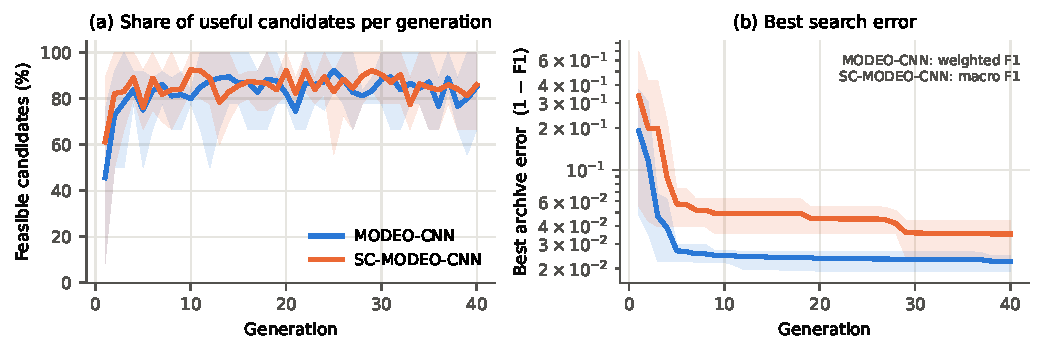
\includegraphics[width=\columnwidth]{fig_search_dynamics.pdf}
\caption{Search dynamics over 40 generations (mean and min--max over 5 seeds). Panel (b) uses weighted F1 for MODEO-CNN and macro F1 for SC-MODEO-CNN.}\label{fig:search}
\end{figure}
\begin{figure}[t]\centering
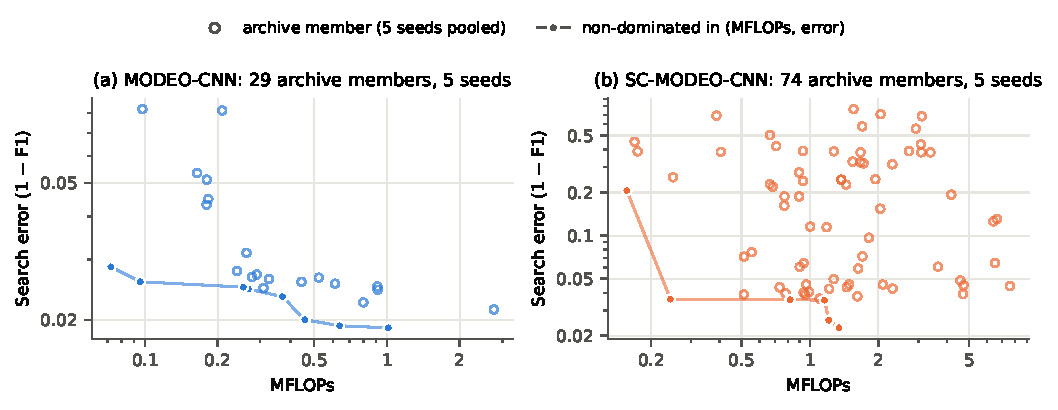
\includegraphics[width=\columnwidth]{fig_pareto_archives.pdf}
\caption{Final archives (5 seeds pooled) projected on MFLOPs and search error. SC-MODEO-CNN archives are three-objective fronts, shown here in projection.}\label{fig:archive}
\end{figure}
\begin{figure*}[t]\centering
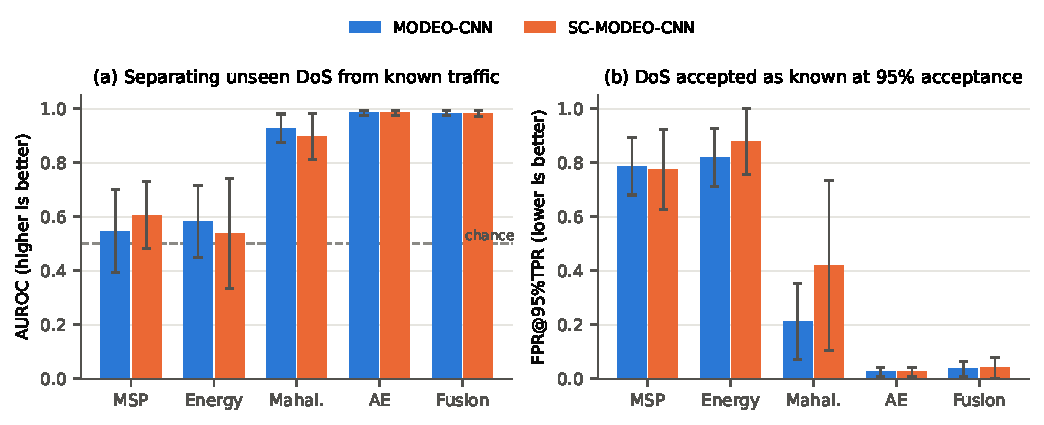
\includegraphics[width=0.8\textwidth]{fig_zero_day_scores.pdf}
\caption{Detecting the unseen DoS attack with five post-hoc scores (mean $\pm$ s.d., 5 seeds).}\label{fig:zeroday}
\end{figure*}
\begin{figure*}[t]\centering
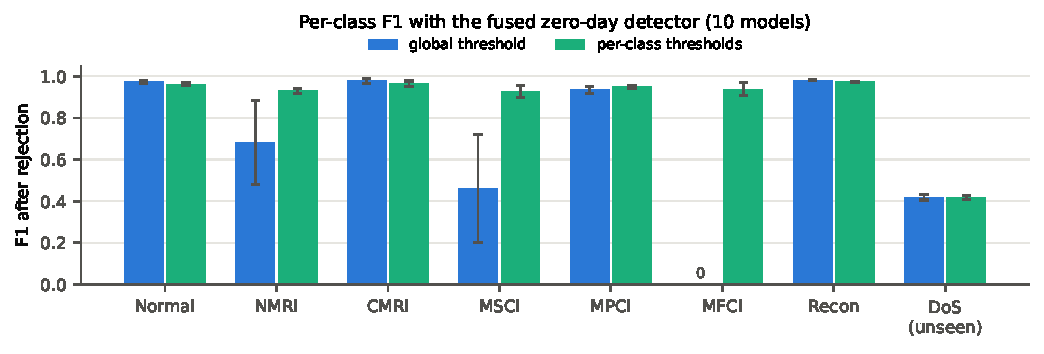
\includegraphics[width=0.8\textwidth]{fig_per_class_thresholds.pdf}
\caption{Per-class F1 after rejection with the fused detector: global vs.\ per-class thresholds (10 models).}\label{fig:perclass}
\end{figure*}

\subsection{Search behaviour}
Figure~\ref{fig:search}(a) shows that, with the feasibility rule, the
search quickly concentrates on useful models: the share of feasible
candidates rises from about 45--60\% in the first generation to about
85\% by generation 5 for both variants. Most of the drop in the best error
happens within the first ten generations (Figure~\ref{fig:search}(b)).
The SC-MODEO-CNN curve lies higher only because macro F1 is a harder
target than weighted F1; it does not indicate worse models, and the two
methods are compared on equal terms in Table~\ref{tab:closed}.

Pooled over five seeds, the final MODEO-CNN archives contain 29 members
and the SC-MODEO-CNN archives 74 (Figure~\ref{fig:archive}). The third
objective explains the difference: it keeps models that separate the
pseudo-unknown well even when they are neither the smallest nor the most
accurate.



\begin{figure}[t]\centering
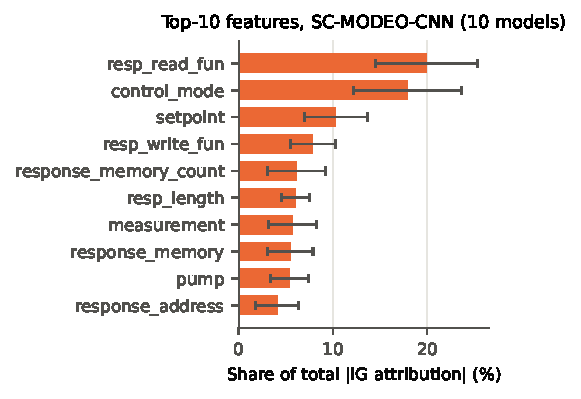
\includegraphics[width=0.85\columnwidth]{fig_feature_importance.pdf}
\caption{Top-10 features by Integrated Gradients attribution (10 SC-MODEO-CNN models).}\label{fig:topfeat}
\end{figure}
\begin{figure}[t]\centering
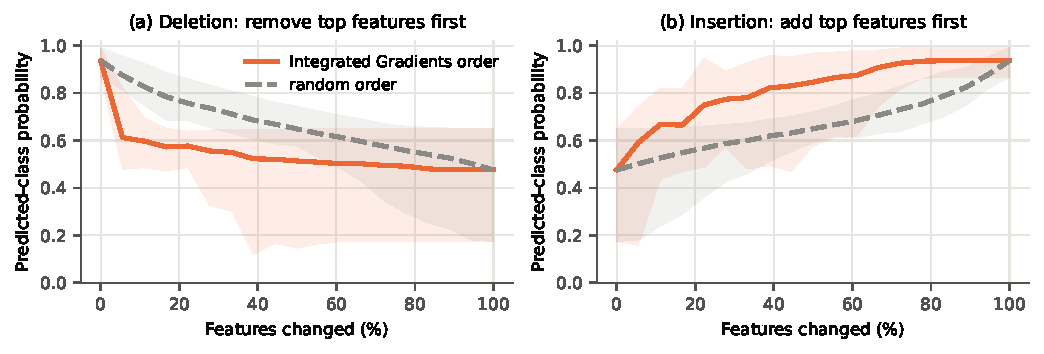
\includegraphics[width=\columnwidth]{fig_faithfulness.pdf}
\caption{Deletion and insertion curves: attribution order vs.\ random order.}\label{fig:delins}
\end{figure}

\subsection{Closed-set classification}
SC-MODEO-CNN reaches a macro-F1 of $0.977 \pm 0.004$ against
$0.974 \pm 0.005$ for MODEO-CNN (Table~\ref{tab:closed}). With $p = 0.125$,
this is a trend rather than a significant improvement. Model size is more
consistent across seeds: $1.34 \pm 0.21$ MFLOPs against $1.07 \pm 1.00$.
The hand-designed CNN (0.980) and the LSTM (0.978) perform on par with
both searched models. A likely reason is that candidates are ranked after
only five epochs on 30\% of the data, which makes the fitness estimates
noisy. The search nevertheless offers an automatic design process and a
set of models covering the trade-off between size and accuracy, rather
than a single fixed network.





\subsection{Zero-day detection of DoS}
Scores computed from the classifier output alone fail to detect DoS: MSP
and energy reach AUROC values of only 0.54--0.61, close to chance
(Figure~\ref{fig:zeroday}). The Mahalanobis score on the embedding is much
better, with AUROC 0.928 for MODEO-CNN and 0.897 for SC-MODEO-CNN, yet it
still accepts 21--42\% of DoS records as known traffic
(Table~\ref{tab:zeroday}). Adding the autoencoder and fusing the scores
raises AUROC to 0.98 and lowers FPR@95 to about 0.04, so roughly ten times
fewer DoS records are missed. However, the fused score performs about the
same as the autoencoder alone, which means the gain comes from the
autoencoder and the embedding adds little for DoS.

Thresholding matters as much as the score itself. With a single global
threshold, rare known classes are rejected too often: MSCI reaches an F1
of only 0.46, MFCI 0.00 and NMRI 0.68, and open-set macro-F1 stays at
0.66--0.69 (Figure~\ref{fig:perclass}). With per-class thresholds, these
rise to 0.93, 0.94 and 0.93, open-set macro-F1 reaches 0.88--0.89 and 97\%
of DoS records are detected. The F1 for DoS itself is only 0.42, because
DoS makes up just 1.9\% of the traffic: the 5\% false-alarm rate on known
traffic produces more false alerts than there are true DoS alarms. In
practice, an operator would choose a stricter operating point.



\subsection{Ablation study}
Table~\ref{tab:ablation} isolates each component. Removing $f_3$ lowers
both macro-F1 (0.962) and Mahalanobis AUROC (0.883). Removing the loss
gene leaves F1 nearly unchanged but produces models about 3.5 times
larger (4.68 against 1.34 MFLOPs). With the easy pseudo-unknown (Recon),
$f_3$ is always zero, so the third objective provides no signal at all.
Two results call for caution. In 16 of 20 runs the search chose an
imbalance-aware loss, which matches the 80\% expected by chance (four of
the five loss options are imbalance-aware), so we do not claim a
preference. Also, $f_3$ learned on CMRI did not beat MODEO-CNN on DoS
(Mahalanobis AUROC 0.897 against 0.928), indicating that separability
learned on a command-injection attack does not transfer to DoS.





\subsection{Explainability}
The attributions are faithful to the models (Table~\ref{tab:xai},
Figure~\ref{fig:delins}). Removing the top-attributed features first
lowers the predicted-class probability faster than random removal
(deletion AUC 0.54 against 0.66), and adding them first raises it faster
(insertion AUC 0.82 against 0.67). Rankings are also fairly stable across
models, with Kendall~$\tau$ of 0.72 for IG and 0.68 for GradientSHAP, and
a top-5 overlap of 0.63--0.64. The most important features are
\texttt{resp\_read\_fun} (20\% of total attribution), \texttt{control\_mode}
(18\%) and \texttt{setpoint} (10\%) (Figure~\ref{fig:topfeat}). These
match the attack mechanics: function-code fields relate to function-code
and command injection, setpoint and control mode to state and parameter
injection, and the measurement field to response injection.


% ---------------------------------------------------------------------
\section{Discussion and Limitations}\label{sec:discussion}

Three choices worked well. Separating detection, handled by the
autoencoder and the embedding distance, from classification made zero-day
detection far more reliable than relying on classifier confidence.
Per-class calibration of thresholds was what turned a good score into
usable open-set detection, because it stopped rare known attacks from
being rejected. The changes to the search itself mainly improved accuracy
and model size.

Other parts did not work as hoped. The zero-day objective, learned on a
single attack type, did not carry over to DoS, and the closed-set gain
was small. Two directions may help: using several pseudo-unknown classes
during search, or replacing the AUROC-based $f_3$ with a distance-based
objective that directly shapes the embedding.

The study has several limitations. Only one unseen attack (DoS) was
evaluated. With five seeds, no comparison can reach significance at
$p < 0.05$. The search budget was reduced relative to the original paper.
Results come from a single dataset, and should be confirmed on others
such as Edge-IIoTset~\cite{ferrag2022edge} and BoT-IoT~\cite{koroniotis2019bot}.
Finally, for rare unknown attacks, any fixed operating point trades
detections against false alarms, and that choice must be made by the
operator.


% ---------------------------------------------------------------------
\section{Conclusion}\label{sec:conclusion}

Intrusion detectors produced by architecture search for IIoT, such as
MODEO-CNN, handle class imbalance poorly, cannot recognise attacks absent
from training, and give no explanation for their alerts. SC-MODEO-CNN
addresses these gaps with an imbalance-aware search that includes a
zero-day objective, a fused detector with per-class thresholds and
verified attribution-based explanations. On Gas Pipeline it reaches a
macro-F1 of 0.977, misses about ten times fewer unseen DoS records and
raises open-set macro-F1 to 0.88--0.89. Future work will apply a
leave-one-attack-out protocol to all attack classes, use more seeds, add
a second dataset and run the search at the full budget.

\bibliographystyle{ieeetr}
\bibliography{refs}

\end{document}
